\documentclass[a4paper,12pt]{article}

\usepackage[utf8]{inputenc}
\usepackage[T1]{fontenc}
\usepackage[french]{babel}
\usepackage{geometry}
\geometry{a4paper, margin=2.5cm}
\usepackage{graphicx}
\usepackage{hyperref}

\title{Rapport Projet Planning}
\author{Emad BA GUBAIR, Tom BARTIER, André MARÇAIS, Yann ROBLIN}
\date{\today}

\begin{document}

\maketitle

\tableofcontents
\newpage
\section{Introduction}
Ce document présente le projet PNG (Planning Nouvelle Génération) qui a été réalisé par un groupe d'étudiants
de M1 Maths Info dans le cadre du cours de modéliatione gestion de projet de madame Murisasco, ainsi que 
Jérémy Maloffre et Laurent Loiseau. Le projet consiste à développer une application
de gestion de planning pour une université en Java avec une interface graphique en JavaFX et une base de données
relationnelle. Le groupe a décidé d'utiliser une base de données PostgreSQL ainsi que l'implémentation de JPA Hibernate.
Le projet s'est déroulé sur 4 Sprints d'une semaine et un dernier Sprint de deux semaines pour une équipe de 
4 étudiants.
\section{Présentation des membres du groupe}
Le groupe est composé de 4 membres :\\
Tom Bartier : En charge de la direction du projet ainsi que du bon fonctionnement l'équipe, aussi en charge de la partie
Backend du projet (mise en place de la BD, écriture des classes des objets de la BD, des Repositories pour interagir avec les objets, 
des requêtes JPQL).\\\\
Yann ROBLIN :   \\\\%TODO
Emad BA GUBAIR :   \\\\%TODO
André MARÇAIS :  \\\\%TODO

\section{Glossaire}
\begin{itemize}
    \item Utilisateur : Personne utilisant l'application
    \item Étudiant : Personne suivant des cours
    \item Professeur aussi équivalent à "enseignant" : Personne enseignant des cours
    \item Administrateur : Personne gérant les comptes
    \item Visiteur : Personne non connectée
    \item Secrétaire : Personne gérant les absences
    \item Responsable EDT : Personne gérant l'emploi du temps
    \item Module : Ensemble de cours sur un même thème
    \item Groupe : Ensemble d'étudiants suivant les mêmes cours
    \item Salle : Lieu où se déroulent les cours
    \item Cours aussi équivalent à "créneau" ou "séance" : un cours est un moment réservé dans l'emploi du temps pour un module donné
    \item EDT : Emploi du temps
    \item iCal : Format de fichier pour les calendriers
    \item PDF : Format de fichier pour les documents
    \item Note : Informations supplémentaires sur un cours
    \item Note personnelle : Note ajoutée par un utilisateur sur un cours visible uniquement par lui-même
    \item Note générale : Note ajoutée par un professeur sur un cours visible par tous
\end{itemize}

\section{Expression du besoin et la restitution des interviews}
Identifions les différents types d'utilisateurs de l'application :\\
L'étudiant : Il doit pouvoir consulter son emploi du temps, ses notes personnelles et générales. Il doit également pouvoir ajouter des notes personnelles sur ses cours.\\
Le professeur : Il doit pouvoir consulter son emploi du temps, celui des groupes et des salles, effectuer des demandes d'ajout ou de mofification de cours, 
consulter et modifier les notes générales et sa note personnelle.\\
Le responsable EDT : Il doit pouvoir consulter l'emploi du temps des groupes, des salles et des modules effectuer des demandes 
ajouter et modifier des cours et consulter et accepter ou refuser les différentes demandes des professeurs.\\
Nous avions aussi pensé à d'autres utilisateurs comme le secrétaire qui gère les absences,
l'administrateur qui gère les comptes et le visiteur qui n'est pas connecté, mais nous n'avons pas eu le temps de les implémenter.\\

\section{Exigences}
\subsection{Login}

\begin{itemize}
    \item \textbf{EX\_LOGIN\_001: Créer un compte} \\
    L'administrateur doit pouvoir créer des comptes élève, professeur, et responsable d'emploi du temps.

    \item \textbf{EX\_LOGIN\_002: Se connecter} \\
    L'utilisateur doit pouvoir se connecter qu'il soit élève, professeur ou responsable d'emploi du temps sur une unique interface.

    \item \textbf{EX\_LOGIN\_003: Consulter anonymement} \\
    Les utilisateurs doivent pouvoir accéder anonymement à l'application avec des restrictions.
\end{itemize}

\subsection{Fonctionnalités générales}

\begin{itemize}
    \item \textbf{EX\_BASE\_FEATURES\_001: Consulter emploi du temps personnel} \\
    Les utilisateurs connectés doivent pouvoir consulter leur emploi du temps respectif.

    \item \textbf{EX\_BASE\_FEATURES\_002: Consulter emploi du temps salles} \\
    Les utilisateurs connectés ainsi que les anonymes doivent pouvoir consulter l'emploi du temps des salles.

    \item \textbf{EX\_BASE\_FEATURES\_003: Consulter emploi du temps d'un groupe} \\
    Les utilisateurs connectés doivent pouvoir consulter l'emploi du temps d'un groupe.

    \item \textbf{EX\_BASE\_FEATURES\_004: Consulter emploi du temps d'un professeur} \\
    Les utilisateurs connectés doivent pouvoir consulter l'emploi du temps d'un professeur.

    \item \textbf{EX\_BASE\_FEATURES\_005: Consulter emploi du temps d'un module} \\
    Les utilisateurs connectés doivent pouvoir consulter l'emploi du temps d'un module.

    \item \textbf{EX\_BASE\_FEATURES\_006: Export iCal} \\
    Les utilisateurs connectés doivent pouvoir exporter leur emploi du temps au format iCal.

    \item \textbf{EX\_BASE\_FEATURES\_007: Consulter nombre d'heures par module} \\
    Les utilisateurs peuvent consulter le nombre d'heures d'un module.

    \item \textbf{EX\_BASE\_FEATURES\_008: Consulter le nombre d'heures total} \\
    Les utilisateurs peuvent consulter le nombre d'heures total d'un groupe ou d'un étudiant.

    \item \textbf{EX\_BASE\_FEATURES\_009: Télécharger PDF} \\
    Les utilisateurs peuvent télécharger le planning au format PDF.

    \item \textbf{EX\_BASE\_FEATURES\_010: Rajouter une note sur un cours} \\
    Les professeurs peuvent rajouter une petite note sur un cours.

    \item \textbf{EX\_BASE\_FEATURES\_011: Consulter les notes de cours} \\
    Les étudiants et les professeurs peuvent consulter les petites notes de cours.

    \item \textbf{EX\_BASE\_FEATURES\_012: Création de notes personnelles} \\
    Les notes personnelles sont visibles uniquement par leur auteur. Par exemple, un étudiant peut noter ce qui a été fait ce jour-là si le professeur ne l'a pas noté.
\end{itemize}

\subsection{Report/annulation de cours}

\begin{itemize}
    \item \textbf{EX\_REPORT\_001: Reporter un cours} \\
    Les professeurs doivent pouvoir demander au responsable de l'emploi du temps de reporter un cours.

    \item \textbf{EX\_REPORT\_002: Annuler un cours} \\
    Les professeurs doivent pouvoir demander au responsable de l'emploi du temps d'annuler un cours.

    \item \textbf{EX\_REPORT\_003: Contacter responsable} \\
    Un professeur peut contacter automatiquement le responsable de l'emploi du temps pour réserver une salle à une heure pour un cours.

    \item \textbf{EX\_REPORT\_004: Consulter cours reporté/annulé} \\
    Les utilisateurs connectés peuvent voir la liste des cours reportés ou annulés.
\end{itemize}

\subsection{Absences}

\begin{itemize}
    \item \textbf{EX\_ABSENCES\_001: Faire l'appel} \\
    Les professeurs peuvent faire l'appel pendant un cours.

    \item \textbf{EX\_ABSENCES\_002: Consulter absences sur un cours} \\
    Les professeurs peuvent consulter les élèves qu'ils ont noté comme absents à un cours.

    \item \textbf{EX\_ABSENCES\_003: Étudiant consulter absences} \\
    Les étudiants peuvent consulter leurs absences passées.

    \item \textbf{EX\_ABSENCES\_004: Prévenir d'un retard/absence} \\
    Les étudiants peuvent prévenir les professeurs s'ils ont un retard ou une absence prévue.
\end{itemize}

\subsection{Fonctionnalités Responsable EDT}

\begin{itemize}
    \item \textbf{EX\_RESP\_001: Ajouter un cours} \\
    Le responsable EDT doit pouvoir insérer un nouveau cours avec les informations qui le concernent dans la base de données de l'application. Il peut en définir les droits de modification et copier-coller un cours existant.

    \item \textbf{EX\_RESP\_002: Modifier un cours} \\
    Le responsable EDT doit pouvoir modifier un cours (heure, professeur, module, salle) s'il a les droits de modification sur ce cours.

    \item \textbf{EX\_RESP\_003: Supprimer un cours} \\
    Le responsable EDT doit pouvoir supprimer un cours s'il a les droits de modification sur ce dernier.

    \item \textbf{EX\_RESP\_004: Accepter demande de modification de cours} \\
    Le responsable EDT doit pouvoir accepter une demande de report de cours effectuée par un professeur.

    \item \textbf{EX\_RESP\_005: Reporter un cours} \\
    Le responsable EDT doit pouvoir reporter un cours.

    \item \textbf{EX\_RESP\_006: Annuler un cours} \\
    Le responsable EDT doit pouvoir annuler un cours.
\end{itemize}

\section{Conception UML générale de l’application}
Voici quelques diagrammes concernant l'organisation générale de l'application (voir figures \ref{fig:uml_uc} et \ref{fig:uml_classes}).\\
Le schéma de la base de données est presque identique au diagramme de classes, il y a juste les notes personnelles, les demandes de cours ainsi que toutes les tables de liaison 
pour les liens n-m en plus.\\
\begin{figure}[h]
    \centering
    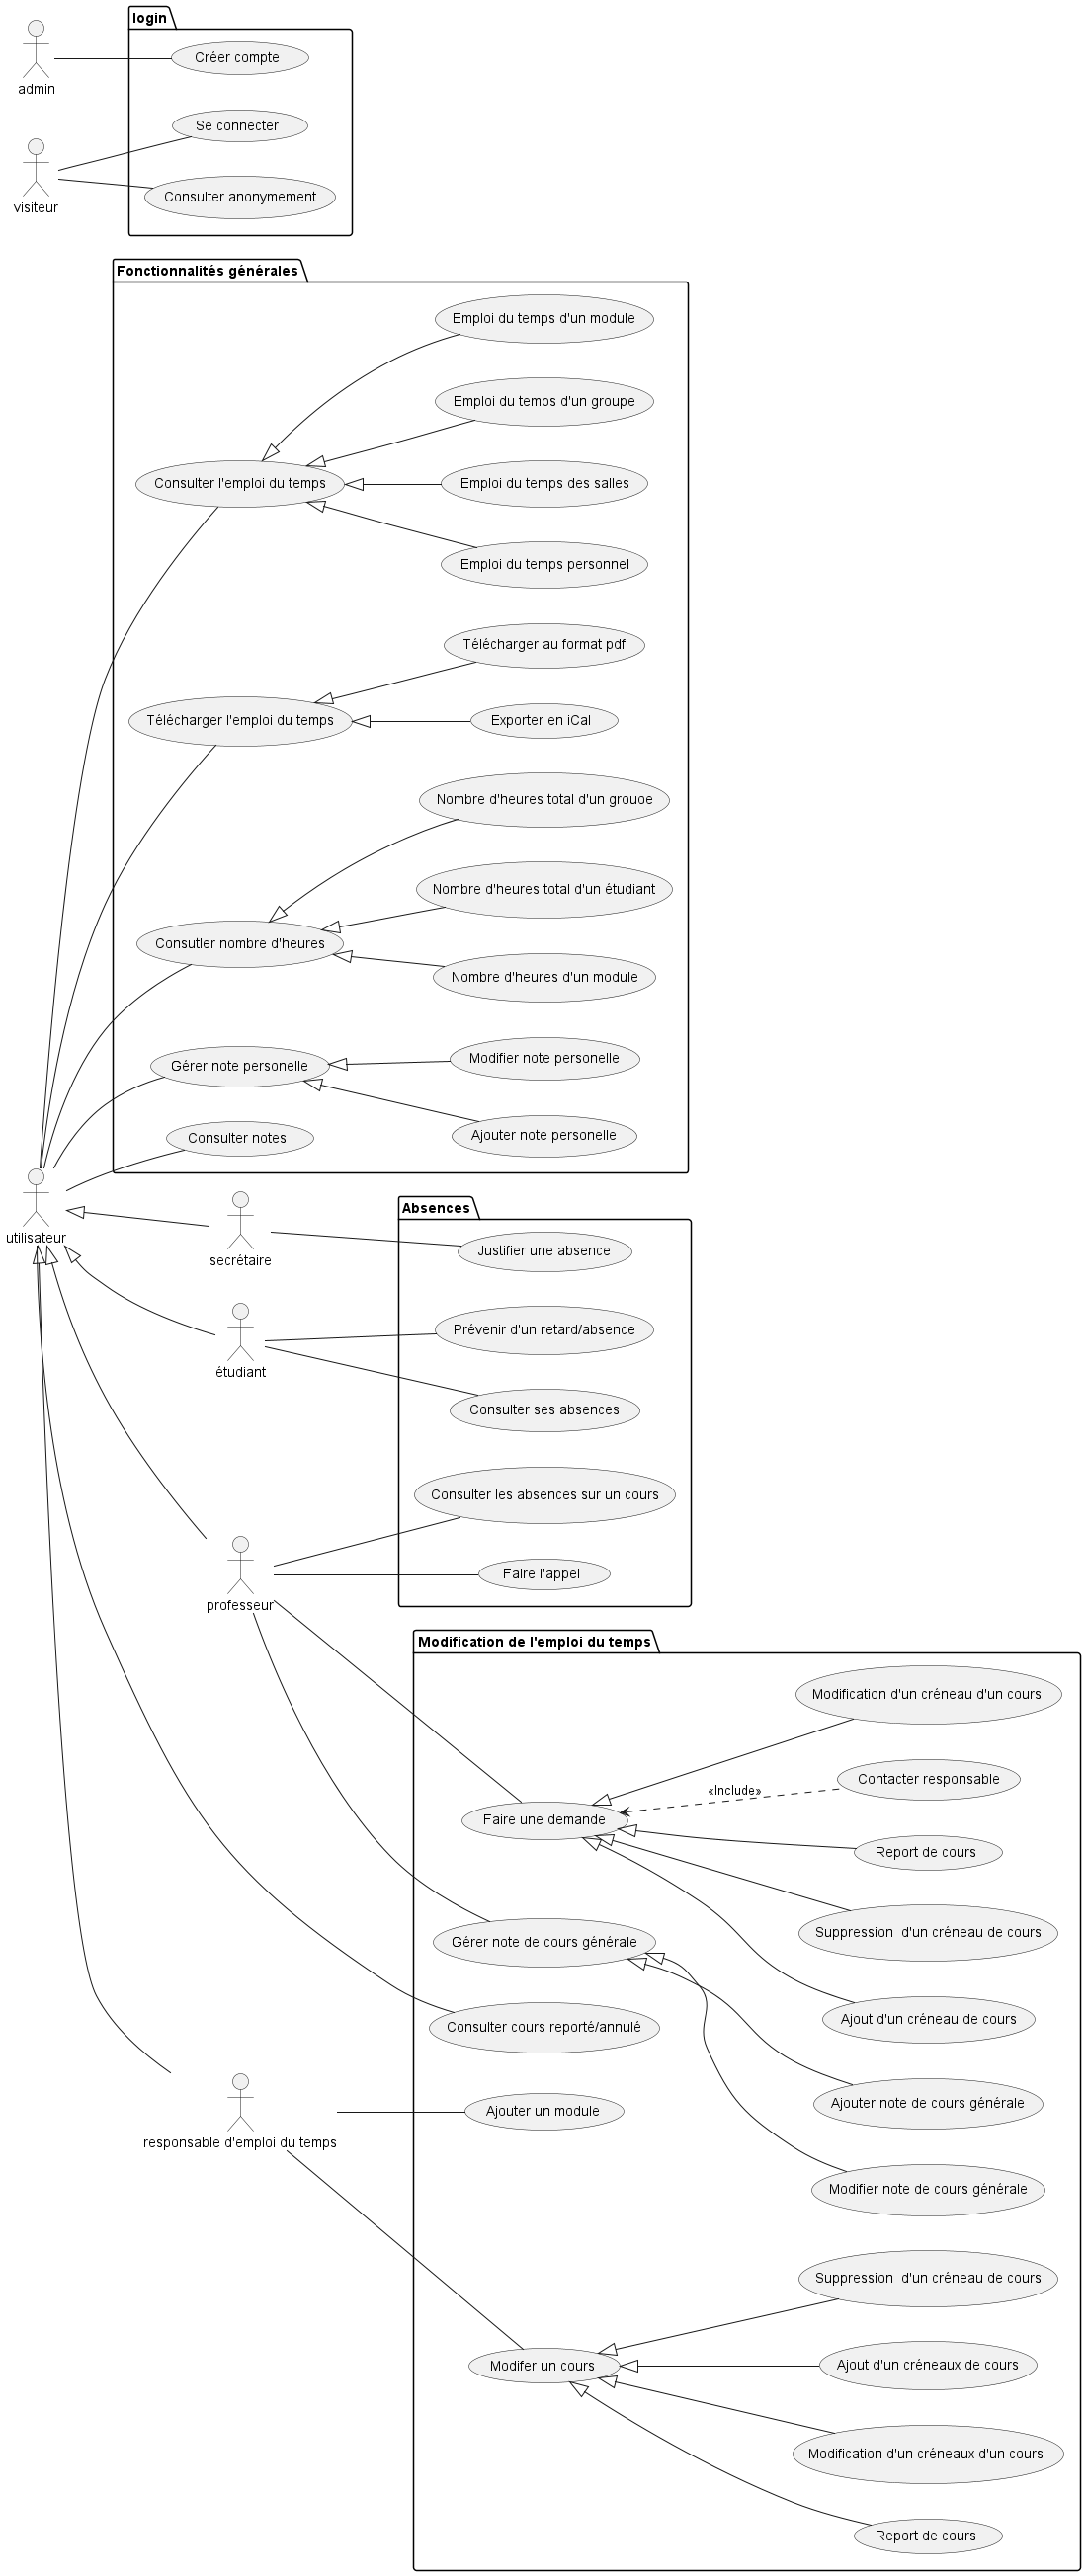
\includegraphics[width=0.65\textwidth]{UC.png}
    \caption{Diagramme de cas d'utilisations}
    \label{fig:uml_uc}
\end{figure}

\begin{figure}[h]
    \centering
    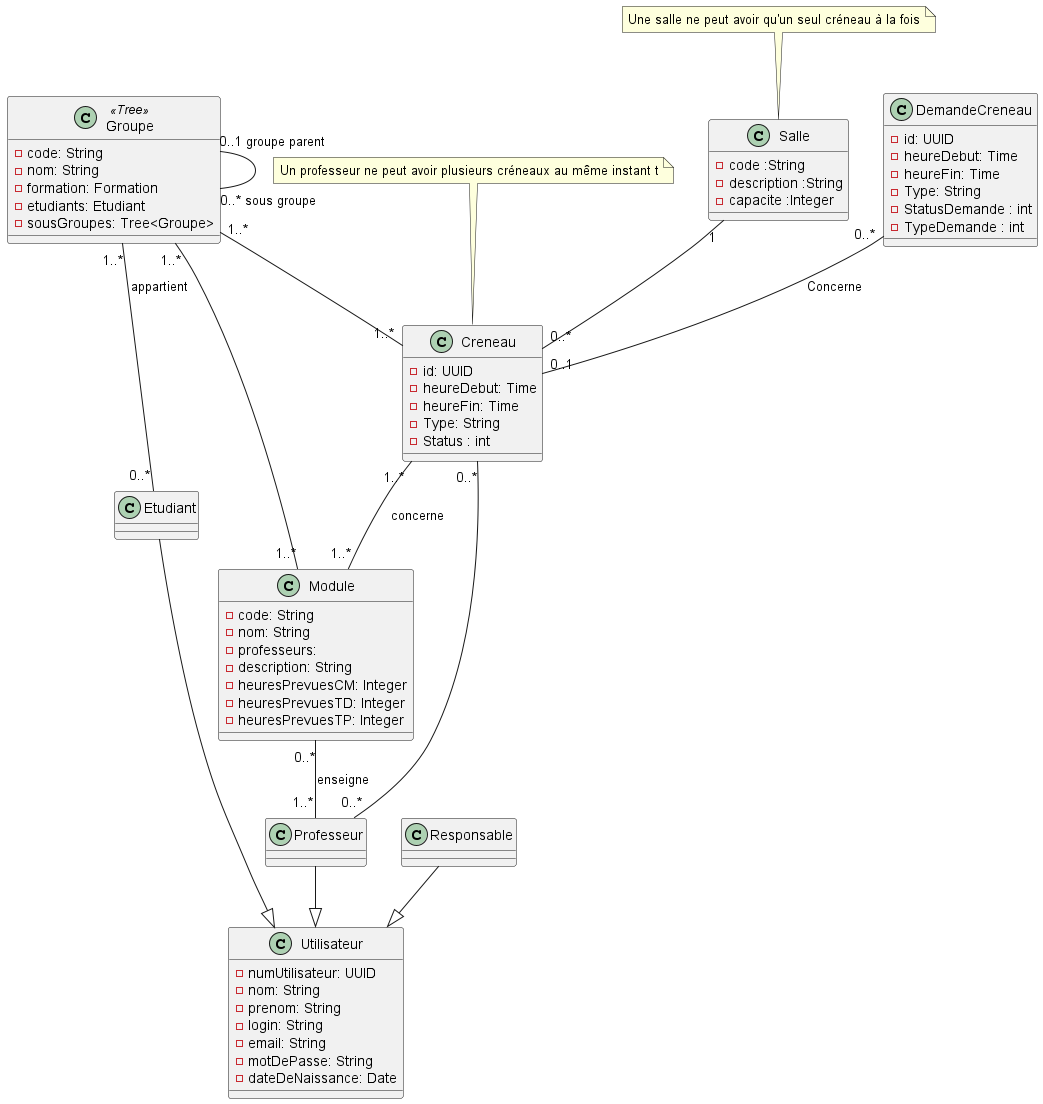
\includegraphics[width=0.65\textwidth]{classes.png}
    \caption{Diagramme de classes}
    \label{fig:uml_classes}
\end{figure}

\section {Spécifications de quelques UC}

\subsection{"UC04 Consulter emploi du temps personnel"}
Description : L'utilisateur connecté consulte son emploi du temps personnel sur la semaine voulue.\\
Acteur : Utilisateur \\
Déclencheur : L'utilisateur arrive sur la page d'accueil ou clique sur "Mon emploi du temps"\\
Pré-Condition : L'utilisateur est connecté\\
Post-Condition : L'emploi du temps de l'utilisateur et de la semaine choisie est affiché\\

Scénario nominal\\
1. L'utilisateur clique sur le bouton "Mon EDT"\\
2. Le système affiche l'emploi du temps de l'utilisateur sur une semaine\\

Scénarios alternatifs\\
Choix semaine\\
3. a L'utilisateur clique sur le numéro de la semaine qui l'intéresse\\
4. a Le système affiche l'EDT de l'utilisateur sur la semaine choisie\\

\subsection{UC03 "Consulter l'emploi du temps par salles"}
Description : L'utilisateur connecté consulte l'emploi du temps de la salle voulue sur la semaine voulue.\\
Acteur : Utilisateur \\
Déclencheur : L'utilisateur clique sur "Salle"\\
Pré-Condition : L'utilisateur est connecté\\
Post-Condition : L'emploi du temps de la salle et de la semaine choisie est affiché
\\

Scénario nominal\\
1. L'utilisateur clique sur le bouton "Salles"\\
2. Le système affiche la liste des salles\\
3. L'utilisateur clique sur le nom de la salle qui l'intéresse\\
4. Le système affiche l'emploi du temps de la salle sur une semaine\\

Scénarios alternatifs\\
Changer salle affichée\\
3. L'utilisateur clique sur le nom de la salle\\
4. Le système affiche toutes les salles\\
5. L'utilisateur clique sur le nom de la salle qui l'intéresse\\
6. Le système affiche l'EDT de la salle sur la semaine\\

Choix semaine\\
3. L'utilisateur clique sur le numéro de la semaine qui l'intéresse\\
4. Le système affiche l'EDT de la salle sur la semaine choisie\\

Diagramme d'activités de l'UC03 : voir figure \ref{fig:act_03}.\\
\begin{figure}[h]
    \centering
    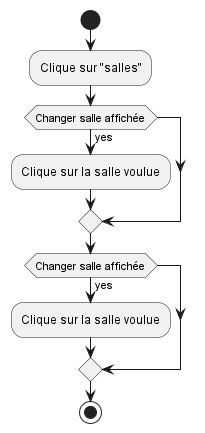
\includegraphics[width=0.2\textwidth]{Diag_activites_UC03.png}
    \caption{Diagramme d'activités UC03}
    \label{fig:act_03}
\end{figure}

\subsection{UC11 "Ajouter un cours"}
Description : le responsable ajoute un créneau cours dans l'emploi du temps\\
Acteur : Responsable d'EDT\\
Déclencheur : Le responsable clique sur un créneau vide ou sur le bouton "Ajouter nouveau cours"\\
Pré-Condition : Le responsable est connecté et un créneau vide est disponible\\
Post-Condition : Le créneau de cours a été crée dans l'emploi du temps\\

Scénario nominal : \\
1. Le responsable clique sur le bouton "Ajouter un cours"\\
2. Le système affiche une fenêtre pour rentrer les informations du cours\\
3. Le responsable clique sur le bouton "Module"\\
4. Le système affiche la liste des modules\\
5. Le responsable clique sur le module du cours\\
6. Le responsable clique sur le bouton "Professeur"\\
7. Le système affiche la liste des professeurs\\
8. Le responsable clique sur le professeur du cours\\
9. Le responsable clique sur le bouton "Horaire"\\
10. Le système affiche la liste des jours et heures\\
11. Le responsable clique sur le jour et l'heure de début et de fin du cours\\
12. Le responsable clique sur le bouton "Salle"\\
13. Le système affiche la liste des salles disponibles\\
14. Le responsable clique sur la salle du cours\\
15. Le responsable clique sur le bouton "Valider"\\
16. Le système affiche le cours ajouté\\

Scénario alternatif\\
15. Le responsable clique sur le bouton "Propager"\\
16. Le système affiche deux menus déroulants de semaine\\
17. Le responsable sélectionne la semaine de début et la semaine de fin\\
18. Le responsable clique sur le bouton "Valider"\\
19. Le système affiche les cours ajoutés\\

Scénario d'exception\\
15. Le responsable clique sur le bouton "Annuler"\\
16. Le système ferme la fenêtre\\

Voir digramme d'activités de l'UC11 figure \ref{fig:act_011}.\\

\begin{figure}[h]
    \centering
    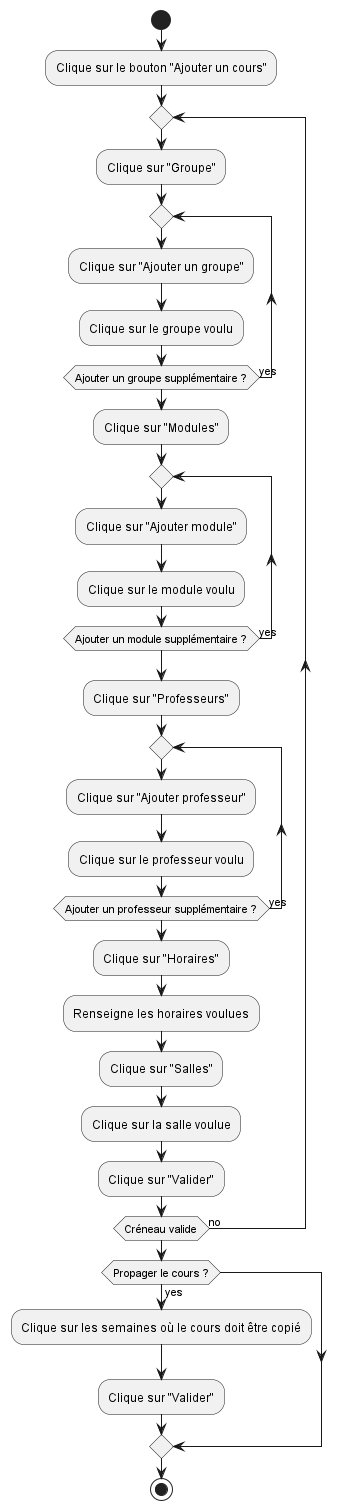
\includegraphics[width=0.35\textwidth]{Diag_activites_UC11.png}
    \caption{Diagramme d'activités UC11}
    \label{fig:act_011}
\end{figure}

\section {Autres scénarios}

\subsection{Package Login}
\subsubsection{UC01 Se connecter}
\paragraph{Scénario Nominal}
\begin{enumerate}
    \item Le visiteur rentre son login et son mot de passe.
    \item Le visiteur clique sur le bouton "Connexion".
    \item \textit{[Identifiants corrects]}.
    \item Le système affiche la page d'accueil de l'utilisateur.
\end{enumerate}

\paragraph{Scénario Alternatif}
\begin{enumerate}
    \item[3.a] \textit{[Identifiants incorrects]}.
    \item[4.a] Le système affiche "Identifiants incorrect", l'UC reprend en 1.
\end{enumerate}

\subsubsection{UC02 Consulter anonymement}
\paragraph{Scénario Nominal}
\begin{enumerate}
    \item Le visiteur clique sur le bouton "Connexion anonyme".
    \item Le système affiche l'emploi du temps des salles, voir UC "Emploi du temps des salles".
\end{enumerate}

\subsection{Package Fonctionnalités générales}
\subsubsection{UC03 Consulter emploi du temps des salles}
\paragraph{Scénario Nominal}
\begin{enumerate}
    \item L'utilisateur clique sur le bouton "Salles".
    \item Le système affiche la liste des salles.
    \item L'utilisateur clique sur le nom de la salle qui l'intéresse.
    \item Le système affiche l'emploi du temps de la salle sur une semaine.
\end{enumerate}

\paragraph{Scénarios Alternatifs}
\subparagraph{Changer salle affichée}
\begin{enumerate}
    \item[3.a] L'utilisateur clique sur le nom de la salle.
    \item[4.a] Le système affiche toutes les salles.
    \item[5.a] L'utilisateur clique sur le nom de la salle qui l'intéresse.
    \item[6.a] Le système affiche l'EDT de la salle sur la semaine.
\end{enumerate}

\subparagraph{Choix semaine}
\begin{enumerate}
    \item[3.b] L'utilisateur clique sur le numéro de la semaine qui l'intéresse.
    \item[4.b] Le système affiche l'EDT de la salle sur la semaine choisie.
\end{enumerate}

\subsubsection{UC04 Consulter emploi du temps personnel}
\paragraph{Prérequis} L'utilisateur est connecté.

\paragraph{Scénario Nominal}
\begin{enumerate}
    \item L'utilisateur clique sur le bouton "Mon EDT".
    \item Le système affiche l'emploi du temps de l'utilisateur sur une semaine.
\end{enumerate}

\paragraph{Scénarios Alternatifs}
\subparagraph{Choix semaine}
\begin{enumerate}
    \item[3.a] L'utilisateur clique sur le numéro de la semaine qui l'intéresse.
    \item[4.a] Le système affiche l'EDT de l'utilisateur sur la semaine choisie.
\end{enumerate}

\subsubsection{UC05 Consulter emploi du temps d'un groupe}
\paragraph{Prérequis} L'utilisateur est connecté.

\paragraph{Scénario Nominal}
\begin{enumerate}
    \item L'utilisateur clique sur le bouton "Groupes".
    \item Le système affiche la liste des groupes.
    \item L'utilisateur clique sur le nom du groupe qui l'intéresse.
    \item Le système affiche l'emploi du temps du groupe sur une semaine.
\end{enumerate}

\paragraph{Scénarios Alternatifs}
\subparagraph{Changer groupe affiché}
\begin{enumerate}
    \item[3.a] L'utilisateur clique sur le nom du groupe.
    \item[4.a] Le système affiche tous les groupes.
    \item[5.a] L'utilisateur clique sur le nom du groupe qui l'intéresse.
    \item[6.a] Le système affiche l'EDT du groupe sur la semaine.
\end{enumerate}

\subparagraph{Choix semaine}
\begin{enumerate}
    \item[3.b] L'utilisateur clique sur le numéro de la semaine qui l'intéresse.
    \item[4.b] Le système affiche l'EDT du groupe sur la semaine choisie.
\end{enumerate}

\subsubsection{UC06 Consulter emploi du temps d'un module}
\paragraph{Prérequis} L'utilisateur est connecté.  
TODO: Décider qui peut consulter les modules.

\paragraph{Scénario Nominal}
\begin{enumerate}
    \item L'utilisateur clique sur le bouton "Modules".
    \item Le système affiche la liste des modules.
    \item L'utilisateur clique sur le nom du module qui l'intéresse.
    \item Le système affiche la liste des cours du module.
\end{enumerate}

\paragraph{Scénarios Alternatifs}
\subparagraph{Changer module affiché}
\begin{enumerate}
    \item[3.a] L'utilisateur clique sur le nom du module.
    \item[4.a] Le système affiche tous les modules.
    \item[5.a] L'utilisateur clique sur le nom du module qui l'intéresse.
    \item[6.a] Le système affiche la liste des cours du module.
\end{enumerate}

\subsubsection{UC07 Ajouter une note personnelle}
\paragraph{Prérequis} L'utilisateur est connecté.

\paragraph{Scénario Nominal}
\begin{enumerate}
    \item L'utilisateur clique sur le cours qui l'intéresse.
    \item Le système affiche une fenêtre pour ajouter une note personnelle.
    \item L'utilisateur rentre sa note.
    \item L'utilisateur clique sur le bouton "Valider".
    \item Le système affiche la note sur le cours.
\end{enumerate}

\paragraph{Scénario d'Exception}
\begin{enumerate}
    \item[4.a] L'utilisateur clique hors de la fenêtre.
    \item[5.a] Le système ne prend pas en compte la note.
\end{enumerate}

\subsubsection{UC08 Modifier une note personnelle}
\paragraph{Prérequis} L'utilisateur est connecté et une note est déjà présente.

\paragraph{Scénario Nominal}
\begin{enumerate}
    \item L'utilisateur clique sur le cours qui l'intéresse.
    \item Le système affiche la fenêtre de la note personnelle.
    \item L'utilisateur modifie sa note.
    \item L'utilisateur clique sur le bouton "Valider".
    \item Le système affiche la note modifiée sur le cours.
\end{enumerate}

\paragraph{Scénario d'Exception}
\begin{enumerate}
    \item[3.a] L'utilisateur clique hors de la fenêtre.
    \item[4.a] Le système ne modifie pas la note.
\end{enumerate}

\subsubsection{UC09 Consulter notes}
\paragraph{Prérequis} L'utilisateur est connecté.

\paragraph{Scénario Nominal}
\begin{enumerate}
    \item L'utilisateur clique sur le cours qui l'intéresse.
    \item Le système affiche la note personnelle de l'utilisateur et la note générale.
\end{enumerate}

\subsection{Package Modification de l'emploi du temps}

\subsubsection{UC11 Ajouter un cours}
\paragraph{Prérequis} Le responsable est connecté.

\paragraph{Scénario nominal}
\begin{enumerate}
    \item Le responsable clique sur le bouton "Ajouter un cours".
    \item Le système affiche une fenêtre pour rentrer les informations du cours.
    \item Le responsable clique sur le bouton "Module".
    \item Le système affiche la liste des modules.
    \item Le responsable clique sur le module du cours.
    \item Le responsable clique sur le bouton "Professeur".
    \item Le système affiche la liste des professeurs.
    \item Le responsable clique sur le professeur du cours.
    \item Le responsable clique sur le bouton "Horaire".
    \item Le système affiche la liste des jours et heures.
    \item Le responsable clique sur le jour et l'heure de début et de fin du cours.
    \item Le responsable clique sur le bouton "Salle".
    \item Le système affiche la liste des salles disponibles.
    \item Le responsable clique sur la salle du cours.
    \item Le responsable clique sur le bouton "Valider".
    \item Le système affiche le cours ajouté.
\end{enumerate}

\paragraph{Scénario alternatif}
\begin{enumerate}
    \item[15.] Le responsable clique sur le bouton "Propager".
    \item[16.] Le système affiche deux menus déroulants de semaine.
    \item[17.] Le responsable sélectionne la semaine de début et la semaine de fin.
    \item[18.] Le responsable clique sur le bouton "Valider".
    \item[19.] Le système affiche les cours ajoutés.
\end{enumerate}

\paragraph{Scénario d'exception}
\begin{enumerate}
    \item[15.] Le responsable clique sur le bouton "Annuler".
    \item[16.] Le système ferme la fenêtre.
\end{enumerate}

\subsubsection{UC12 Modification d'un créneau d'un cours}
\paragraph{Prérequis} Le responsable est connecté et un cours est déjà présent.

\paragraph{Scénario nominal}
\begin{enumerate}
    \item Le responsable clique sur le cours qui l'intéresse.
    \item Le système affiche une fenêtre pour modifier les informations du cours.
    \item Le responsable modifie les informations du cours qu'il veut modifier, voir UC "Ajouter un cours".
    \item Le responsable clique sur le bouton "Valider".
    \item Le système affiche le cours modifié.
\end{enumerate}

\subsubsection{UC13 Annulation de cours}
\paragraph{Prérequis} Le responsable est connecté et un cours est déjà présent.

\paragraph{Scénario nominal}
\begin{enumerate}
    \item Le responsable clique sur le cours qui l'intéresse.
    \item Le système affiche les informations du cours (module, professeur, salle, horaires, nom du responsable qui l'a ajouté, jour de dernière modification).
    \item Le responsable clique sur le bouton "Supprimer".
    \item Le système affiche "Voulez-vous vraiment supprimer ce cours ?".
    \item Le responsable clique sur "Oui".
    \item Le système affiche "Cours supprimé".
\end{enumerate}

\paragraph{Scénario d'exception}
\begin{enumerate}
    \item[5.a] Le responsable clique sur "Non".
    \item[6.a] Le système ne supprime pas le cours.
\end{enumerate}

\subsubsection{UC14 Accepter demande de modification de cours}
\paragraph{Prérequis} Le responsable est connecté et une demande de modification est présente.

\paragraph{Scénario nominal}
\begin{enumerate}
    \item Le responsable clique sur le bouton "Demandes de modification".
    \item Le système affiche la liste des demandes de modification.
    \item Le responsable clique sur la demande qui l'intéresse.
    \item Le système affiche les informations du cours (module, professeur, salle, horaires).
    \item Le responsable clique sur le bouton "Accepter".
    \item Le système affiche "Demande acceptée".
\end{enumerate}

\paragraph{Scénario d'exception}
\begin{enumerate}
    \item[5.a] Le responsable clique sur le bouton "Refuser".
    \item[6.a] Le système affiche "Demande refusée".
\end{enumerate}

\subsubsection{UC15 Ajouter un module}
\paragraph{Prérequis} Le responsable est connecté.

\paragraph{Scénario nominal}
\begin{enumerate}
    \item Le responsable clique sur le bouton "Ajouter un module".
    \item Le système affiche une fenêtre pour rentrer les informations du module (id, nom, nombre d'heures).
    \item Le responsable clique sur le bouton "Valider".
    \item Le système affiche le module ajouté.
\end{enumerate}

\paragraph{Scénario d'exception}
\begin{enumerate}
    \item[3.a] Le responsable clique sur le bouton "Annuler".
    \item[4.a] Le système n'ajoute pas le module.
\end{enumerate}

\subsubsection{UC16 Faire une demande de Report de cours}
\paragraph{Prérequis} Le professeur est connecté.

\paragraph{Scénario nominal}
\begin{enumerate}
    \item Le professeur clique sur le cours qui l'intéresse.
    \item Le système affiche les informations du cours (module, professeur, salle, horaires).
    \item Le professeur clique sur le bouton "Reporter".
    \item Le système affiche une fenêtre pour rentrer les informations du report (nouvelle date, nouvelle heure, nouvelle salle).
    \item Le professeur clique sur le bouton "Valider".
    \item Le système affiche "Demande de report envoyée".
\end{enumerate}

\paragraph{Scénario d'exception}
\begin{enumerate}
    \item[5.a] Le professeur clique sur le bouton "Annuler".
    \item[6.a] Le système n'envoie pas la demande de report.
\end{enumerate}

\paragraph{Scénario alternatif}
\begin{enumerate}
    \item[6.b] Les informations du nouveau créneau sont incorrectes (salle occupée ou groupe occupé), le système affiche "Créneau indisponible" avec la raison de l'indisponibilité, l'UC reprend en 4.
\end{enumerate}

\subsubsection{UC17 Ajouter une note de cours générale}
\paragraph{Prérequis} Le professeur est connecté.

\paragraph{Scénario nominal}
\begin{enumerate}
    \item Le professeur clique sur le cours qui l'intéresse.
    \item Le système affiche les informations du cours (module, professeur, salle, horaires).
    \item Le professeur clique sur le bouton "Ajouter une note générale".
    \item Le système affiche une fenêtre pour rentrer la note générale.
    \item Le professeur rentre la note.
    \item Le professeur clique sur le bouton "Valider".
    \item Le système affiche la note générale sur le cours.
\end{enumerate}

\paragraph{Scénario d'exception}
\begin{enumerate}
    \item[6.a] Le professeur clique sur le bouton "Annuler".
    \item[7.a] Le système n'ajoute pas la note.
\end{enumerate}

\subsubsection{UC18 Modifier une note de cours générale}
\paragraph{Prérequis} Le professeur est connecté et une note est déjà présente.

\paragraph{Scénario nominal}
\begin{enumerate}
    \item Le professeur clique sur le cours qui l'intéresse.
    \item Le système affiche les informations du cours (module, professeur, salle, horaires).
    \item Le professeur clique sur le bouton "Modifier la note générale".
    \item Le système affiche la note générale.
    \item Le professeur modifie la note.
    \item Le professeur clique sur le bouton "Valider".
    \item Le système affiche la note modifiée.
\end{enumerate}

\paragraph{Scénario d'exception}
\begin{enumerate}
    \item[6.a] Le professeur clique sur le bouton "Annuler".
    \item[7.a] Le système ne modifie pas la note.
\end{enumerate}


\section{Gestion de projet}
Cette section va présenter la gestion et l'organisation du projet, les outils utilisés, les méthodes de travail, ainsi que les difficultés rencontrées.\\
Le projet est un client en lourd JavaFX qui se connecte à une base de données PostgreSQL dans un container Docker.\\
Nous avons utilisé GitHub pour le versionnage, chaque membre du groupe a une branche et travaille dedans, lorsqu'il a terminé une tâhce, il merge sur la branche dev. En fin de sprint, 
nous nous assurons que la branche dev est fonctionnelle avec toutes nouvelles fonctionnalités ajoutées dans la semaine, puis nous mettons sur la branche main et faisons un tag.\\
Les User Stories réalisées lors de chaque sprint ont été chiffrées sur le document à cette adresse \href{https://docs.google.com/spreadsheets/d/1I3lit2K54TSlTaCaFj2Z68BY6hvbYxaZbvtNGo1Lqdk/edit?usp=sharing}{(lien)}.
Le sprint 0 a été consacré à la mise en place de l'environnement de travail et la création du projet, la rédaction de quelques spécifications et le chiffrage des US du sprint 1.
Au début du sprint 1, nous avons chiffrés les tâches pour le sprint 2 mais nous avions visé trop gros a n'avions pas eu le temps de finir toutes les tâches prévues pour le sprint 1 à la fin de celui-ci.
Nous avons alors décidé à partir de là de ne fixer et chiffrer les tâches d'un sprint qu'au début de celui-ci tout en gardant une vague idée des tâches du prochain sprint.\\
C'est lors du sprint 1 que nous avons commencé à travailler sur le projet. Le groupe s'est mis d'accord sur l'architecture de l'application, de la base de données et des classes de l'application, puis 
Tom a mis en place les classes model et la base de données avec Hibernate, Yann et Emad ont de leur côté commencé à travailler sur le GUI et André a commencé à travailler sur le peuplement de la base avec des
données ressemblant à de vraies données. Un groupe Discord a été mis en place afin que les membres du groupe communiquent entre eux tout au long du sprint, il nous arrivait aussi de discuter pendant la semaine à la fin d'un cours
puis le vendredi matin était dédié à la mise en commun du travail effectué sur la semaine, puis on chiffrait les tâches du sprint qui arrivait, ceci a été l'organisation durant tout le reste du projet.
Par la suite nous avons réussi à effectuer le chiffrage de manière beaucoup plus précise et à respecter les délais de chaque sprint sans pour autant délaisser une partie du travail prévu, 
au final nous avons réussi à implanter presque toutes les fonctionnalités que nous avions considéré comme prioritaires.\\
Concernant les diffcultées rencontrées, il n'y a pas eu de problème majeur, presque aucun soucis de communication ou gestion du groupe, seulement quelques difficultées techniques notemment avec les 
liens n-m de la base de données entre les classes qui ont posé quelques problèmes, nous avons fait l'erreur d'en mettre beaucoup et dans les deux sens ce qui on pensait au début nous ferait gagner du temps pour
faciliter l'accès au données, a au final été ce qui nous a fait perdre le plus de temps pour maintenir l'intégrité de la BD. Un autre point que nous pouvons noter aussi
est qu'au début au sprint 1 nous avions confié à un membre du groupe de s'occuper du peuplement de la base de données avec des données générées aléatoirement ressemblant à de vraies données. N'ayant jamais fait
ce genre de choses nous nous sommes largement trompé sur le chiffrage de cette tâche, qui n'a pas été terminée durant le premier sprint comme prévu initalement, elle a débordée sur le second, puis sur le troisième,
mais voyant que le reste du projet avançait bien, nous nous sommes permis de dédier un membre du groupe entièrement à cette tâche durant tout le projet.\\

\section{Le maquettage de l’application}
Voici un schéma de l'interface principale de l'application telle qu'elle a été imaginée à l'origine (voir figure \ref{fig:maquette}).
\begin{figure}[h]
    \centering
    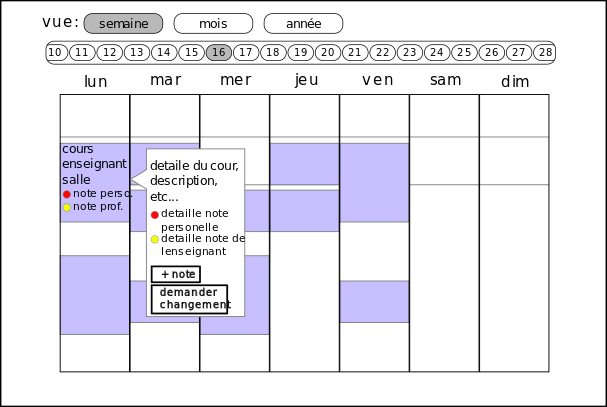
\includegraphics[width=0.8\textwidth]{gui-schema.png}
    \caption{Maquette de l'interface principale de l'application}
    \label{fig:maquette}
\end{figure}
\section{Les perspectives d’évolution de l’application}
Bien que l'application soit fonctionnelle avec quelques fonctionnalités, il reste encore du travail pour l'améliorer.
Dans un premier temps, nous pourrions rajouter un bouton de déconnexion, car pour l'instant, il faut fermer l'application pour se déconnecter.
Nous pourrions aussi rajouter une connexion anonyme pour les utilisateurs qui ne sont pas connectés, mais qui souhaitent consulter l'emploi du temps des salles.
Un rafraîchissement automatique de l'emploi du temps serait une bonne idée car pour l'instant il faut changer de semaine puis revenir sur la semaine pour voir les modifications si il y en eu.
On pourrait aussi rajouter les secrétaires, qui pourraient consulter tous les emplois du temps et gérer les absences des étudiants.
Enfin nous pourrions aussi rajouter une interface d'administration pour gérer les utilisateurs.
\end{document}